\documentclass[a4paper, 11pt]{beamer}
\usepackage{graphicx}
\usepackage{listings}
\usepackage{mathtools}
\usepackage[utf8]{inputenc}
\usepackage{polski}
\usepackage{antiqua}

\usepackage[T1]{fontenc}
\usetheme{Berkeley} %motyw
%Deklaracja kolorów
\begin{document}
%
\title{Symulacja ruchu pociagów}
\author{Prezentację tworzył Adam Mościcki}
\institute{we współpracy z Michał Pluta, Jan Wiśniewski, Edwiń Jarośinski, Paweł Kowalczyk , Margarita Kirillova}
%
\begin{frame} %ramka, nie slajd!!!
\titlepage %strona tytulowa
\end{frame}

\begin{frame}
\tableofcontents
\end{frame}

\section{O projekcie}
\subsection{Treść}
\begin{frame}
\frametitle{Treść}
Należy stworzyć aplikację wizualizującą ruch pociągów. Aplikację należy skonstruować w taki sposób, aby z pliku wczytywany był układ torów z dowolną liczbą skrzyżowań. Układ torów i początkowe rozmieszczenie pociągów powinno być definiowane i wczytywane z pliku. Na skrzyżowaniu domyślnie jest sygnalizacja, ponadto każdy pociąg posiada radar, który pozwala mu określić odległość od innego pociągu jadącego po tym samym torze. Po torowisku może jeździć dowolna liczba pociągów z różnymi prędkościami. Pociągi muszą jeździć tak, aby nie doszło do kolizji. Program musi posiadać moduł sterowania prędkościami pociągów, tak aby nie dochodziło do kolizji! Historia sterowania pociągami(ich prędkości w poszczególnych chwilach czasu i ich zmiany winny być zapamiętywane w pliku). Program musi posiadać możliwość odtwarzania ruchu pociągów zapisanego w pliku z historią.
\end{frame}
\subsection{Założenia}
\begin{frame}
\frametitle{Założenia}
\begin{enumerate}
\item
zastosowanie metodyki scrum z liczbą sprintów 3
\item 
użytkownicy wyszczególnieni to: obserwator, projektant torów, logistyk
\item
podział pracy grupy na 2 podgrupy pracujące niezależnie (niezbyt restrykcyjny, informacje dalej)
\item 
wzorzec projektowy zbliżony do MVC (zwiazane z pkt wyżej)
\end{enumerate}
\end{frame}
\subsection{User stories, sprint 1}
\begin{enumerate}
\begin{frame}
\frametitle{Sprint 1}
\item Jako obserwator chciałbym :
\begin{itemize}
\item b) widzieć jak poruszają się pociągi (must have)
\item d) mieć możliwość zatrzymania symulacji w dowolnej chwili (must have)
\item g) aby stacje były reprezentowane na mapie w postaci graficznej (must have)
\item k) aby program miał możliwość zapisania do pliku przebiegu symulacji (must have)
\end{itemize}
\end{frame}
\begin{frame}
\frametitle{Sprint 1}
\item Jako projektant torów chciałbym :
\begin{itemize}
\item a) mieć możliwość ustawiania stacji w dowolnym punkcie mapy (must have)
\item b) mieć możliwość łączenia stacji torami (jednokierunkowymi lub dwukierunkowymi) (must have)
\item e) projektować skrzyżowania torów (must have)
\item f) ustawiać priotytety przejazdów pociągów na poszczególych skrzyżowaniach (should have)
\item g) mieć możliwość łaczenia wielu odcinków torów i wiele skrzyżowań w segment. Na jednym segmencie nie może znajdować się więcej niż jeden pociąg (nice to have)
\item h) aby plik opisujący mapę miał składnię umożliwiającą względnie nieskomplikowaną edycję mapy (must have)
\end{itemize}
\end{frame}
\begin{frame}
\frametitle{Sprint 1}
\item Jako logistyk chciałbym
\begin{itemize}
\item b) edytując plik wejściowy ustawiać ilość wagonów przed symulacją (should have)
\item h) aby pociąg miał możliwość wyznaczenia właściwej dla siebie trasy na podstawie danych stacji: początkowej i końcowej, a także dowolnej ilości punktów (stacji) "przez" (must have)
\end{itemize}
\end{frame}
\end{enumerate}
\subsection{User stories, sprint 2}
\begin{enumerate}
\begin{frame}
\frametitle{Sprint 2}
\item Jako obserwator chciałbym :
\begin{itemize}
\item a) aby program informował o zablokowaniu się ruchu we wszystkich kierunkach na skrzyżowaniu (możliwe jest wczytanie mapy doprowadzającej do takiej sytuacji) (may have)
\item e) mieć możliwość przyspieszania i zwalniania symulacji (should have)
\item j) aby przy każdym skrzyżowaniu można było sprawdzić stan wszystkich sygnalizacji (needs to have)
\item l) pociągi powinny być sterowane w sposób zapobiegający kolizjom (must have)
\item m) aby symulacja była przedstawiona w czytelnej, ładnej oprawie graficznej (should have)
\item n) aby była możliwość odtworzenia symulacji na podstawie zapisanego pliku (must have)
\end{itemize}
\end{frame}
\begin{frame}
\frametitle{Sprint 2}
\item Jako projektant torów chciałbym :
\begin{itemize}
\item c) mieć możliwość kreowania otoczenia przez bardzo uproszczone elementy, takie jak przeszkody na mapie (may have)
\item d) mieć możliwość ustalenia dowolnej odległości między stacjami (niezależnie od reprezentacji graficznej trasy) (must have)
\end{itemize}
\end{frame}
\begin{frame}
\frametitle{Sprint 2}
\item Jako logistyk chciałbym
\begin{itemize}
\item a) znać odległości pomiędzy poszczególnymi stacjami (must have)
\item g) móc przypisać pociągowi trasę specyfikując punkty (stacje) przez które ma on przejechać (must have)
\end{itemize}
\end{frame}
\end{enumerate}
\subsection{User stories, sprint 3}
\begin{enumerate}
\begin{frame}
\frametitle{Sprint 3}
\item Jako obserwator chciałbym :
\begin{itemize}
\item c) aby można było sprawdzić prędkość poszczególnych pociągów (should have)
\item f) sprawdzać w danej chwili właściwości pociągów (cel podróży i punkty przez) i zadanej trasy (should have)
\item h) aby pociąg zwalniał podczas dojeżdżania do stacji i do skrzyżowań (should have)
\item i) aby pociąg stopniowo zwiększał swoją prędkość ruszając z miejsca (should have)
\end{itemize}
\end{frame}
\begin{frame}
\frametitle{Sprint 3}
\item Jako projektant torów chciałbym :
\begin{itemize}
\item i) aby z programem dostarczony był graficzny edytor mapy (may have)
\item j) tworzyć dowolnie dużą mapę (nice to have)
\end{itemize}
\end{frame}
\begin{frame}
\frametitle{Sprint 3}
\item Jako logistyk chciałbym
\begin{itemize}
\item c) ustawiać maksymalne prędkości poszczególnych pociągów przed symulacją (przez plik wejściowy) (must have)
\item d) aby po dojechaniu pociągu do stacji docelowej generowany był raport zawierający między innymi pokonaną odległość i czas przejazdu (nice to have)
\item e) aby pociąg dostosowywał prędkość do wolniejszego pociągu jadącego przed nim (must have)
\item f) mieć możliwość zadania czasu minimalnego, przez jaki pociąg powinien stać na stacji (nice to have)
\end{itemize}
\end{frame}
\end{enumerate}
\section{Podział abstrakcji}
\subsection{Model i interfejs}
\begin{frame}
\frametitle{Model i interfejs}
%Musze wstawić "Mądry obrazek"
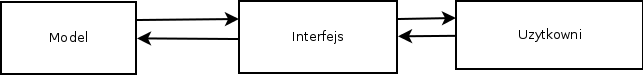
\includegraphics[scale=0.4]{ModelInterf.png}
\begin{itemize}
\item rozwiązanie podobne do szablonu MVC, gdzie kontroler jest częściowo wbudowany w model, a częściowo w interfejs
\item model i interfejs są wzajemnie ortagonalne, tzn. widzą wzajemnie tylko swoje metody zewnętrzne, nie ingerują w implementację wewnętrzną
\item odpowiedzialni za interfejs: Adam(semi master), Edwin, Rita
\item odpowiedzialni za model: Michał (semi master \& grant master), Janek, Paweł
\end{itemize}
\end{frame}
\subsection{Model}
\begin{frame}
\frametitle{Model}
\begin{itemize}
\item graf jako odzwierciedlenie układu torów i skrzyżowań, wierzchołek = skrzyżowanie, krawędź = tor
\item każde skrzyżowanie będzie przechowywać listę skrzyżowań z nim połączonych
\item skrzyżowania będą decydować o dopuszczeniu pociągu na tor - semafory
\item obiekty odzwierciedlające rzeczywistość: train, junction, map, track
\item pociągi będą wyszukiwać kolejne skrzyżowania z użyciem algorytmu Dijkstry
\item przewidywane struktury użytkowe: kopiec(Dijkstra), lista(rep. grafu), możliwe inne, które wyjdą w rzeczywistej realizacji projektu
\end{itemize}
\end{frame}
\begin{frame}
\frametitle{Model}
\framesubtitle{Podział obowiązków}
Janek: 
\begin{itemize}
\item organizacja kontroli ruchu:
\item kontrola sygnalizacji świetlnych na skrzyżowaniach tak, aby uzyskać jak największą wydajność systemu 
\item uwzględnienie priorytetów poszczególnych torów na skrzyżowaniu 
\item zatrzymanie pociągu na czerwonym świetle oraz ruszenie na zielonym 
\item dostosowanie prędkości do warunków jazdy 
\end{itemize}
\end{frame}
\begin{frame}
\frametitle{Model}
\framesubtitle{Podział obowiązków}
Michał: 
\begin{itemize}
\item budowa grafu mapy oraz utworzenie pociągów na podstawie sparsowanych danych z pliku
\item wyznaczanie pożądanej trasy pociągu
\item wykrycie i obsługa sytuacji nietypowych (np. gdy dwa pociągi jadą na siebie)
\item obsługa poleceń wydawanych przez moduł graficzny 
\item zatrzymanie, przyspieszenie symulacji, pobranie informacji o pociągach itp.
\end{itemize}
\end{frame}
\begin{frame}
\frametitle{Model}
\framesubtitle{Podział obowiązków}
Paweł:
\begin{itemize}
\item odczyt pliku z mapą (rozszyfrowanie w wersji kafelkowej) oraz odczyt i zapis plików opisujących przebieg symulacji 
\item kontrola prędkości pociągu 
\item przyspieszanie, hamowanie
\item obsługa przyjazdów pociągów do stacji
\end{itemize}
\end{frame}
\subsection{Interfejs}
\begin{frame}
\frametitle{Interfejs}
\begin{itemize}
\item realizowany z użyciem biblioteki Qt (prawdopodbnie wersja 5) z modułami OpenGL oraz XML
\item w sprincie pierwszym, bardzo uproszczony - do punktów i krawędzi, tj. zwykła interpretacja grafu z kropkami jako pociągami
\item w kolejnych plan utworzenia gotowych kafli, które razem będą dawać dość ciekawy efekt
\item kaflami nazywamy kwadraty będące reprezentacją graficzną podstawowej składowej mapy, które połączone ze sobą w siatce w określony sposób tworzą spójny obraz mapy
\end{itemize}
\end{frame}
\begin{frame}
\frametitle{Interfejs}
\frametitle{Podział obowiązków}
Adam:
\begin{itemize}
\item budowa okna od zera - menu, paski
\item podstawowe przyciski (pauza, start) i suwaki (szybkosc informacji) i ich obsługa
\item komunikacja model <-> interfejs
\item przygotowanie środowiska do wyświetlania symulacji
\item rozszyfrowanie kafli
\item edytor (możliwy po realizacji podstawowych rzeczy)
\end{itemize}
\end{frame}
\begin{frame}
\frametitle{Interfejs}
\frametitle{Podział obowiązków}
Rita:
\begin{itemize}
\item przygotowanie wszystkich tekstur
\item rysowanie obiektów w OpenGL
\item wyświetlanie odpowiednich informacji o właściwościach pociągów, ich statusie, stacjach itp.
\item płynne animacje
\end{itemize}
Edwin:
\begin{itemize}
\item parsowanie plików XML w których jest informacja o symulacji
\item podstawowe sprawdzanie poprawności wprowadzonych danych
\item edytor, zapis do pliku XML
\item powiększanie, przewijanie mapy
\item rozszyfrowanie kafli
\end{itemize}
\end{frame}
\subsection{Przepływ zasobów}
\begin{frame}
\frametitle{Przepływ zasobów}
W zamyśle, kwestia graficzna, w dużej mierze może być zakończona po etapie 2. Aby nie marnować zasobów ludzkich, częścią obowiązków modelowych może być obarczona grupa interfejsowa.
\end{frame}
\subsection{To już jest koniec}
\begin{frame}
\frametitle{Zakończenie}
Dziękujemy.
\end{frame}
\end{document}


